% results.tex

\section{Results}

\subsection{Integrated Vapor Transport}
We use data from the integrated water vapor transport (\emph{IVT}) model\makenote{needs citation}
  of atmospheric rivers as a means of testing these models.  An atmospheric river is a meteorological
  event of local concentration of water vapor in the atmosphere that moves with wind patterns.
  Understanding dependence among extreme events in atmospheric rivers \makenote{finish thought}.

Fitting our models to this data requires some pre-processing.  The marginal distributions of the
  IVT data appear naturally log-normal, which falls into the domain of attraction of a Gumbel
  distribution.  Given that, we can apply thresholding and exceedances over that threshold will
  follow a generalized Pareto distribution.  Our model begins with that assessment.  As estimating
  the Pareto parameters is not yet our focus in this analysis, we choose to apply the threshold
  using the empirical CDF.  That is, for a given $t$, let $b_t = \hat{F}^{-1}(1 - t^{-1})$.  For
  this analysis, we set $t = 20$, indicating the $95$ percentile.  The other parameters of the
  generalized Pareto--the scale parameter $\alpha_t$ and the extremal index $\chi$--are set via
  maximum likelihood.  A fully Bayesian model formulation will allow their varying within a
  distribution, and we hope to eventually allow that.  However, such a model will not lend itself
  to being fitted by MCMC.

After the thresholding and maximum likelihood estimation of the parameters of the Pareto, we scale
  the data to the standard multivariate Pareto.  Dividing each observation by its
  $\mathcal{L}_{\infty}$ norm, we arrive at data on the hypercube.  Data in sequence represents
  observations in time, and these are heavily correlated.  As such, we choose to \emph{decluster}
  the observations by, observing a sequence of observations ${\bf z}$ for which $\inorm{z_i} > 1$
  for each observation in sequence, we keep only the observation with the maximum observed
  $\mathcal{L}_{\infty}$ norm.

We fit the proscribed models to the data via whatever projection is necessary, run the models, and
  use the fitted model parameters to generate posterior predictive distributions--both overall, for
  use with the KL divergence metric, and conditioned on individual observations, for use with the
  posterior predictive loss and energy score metrics.

We have, at our disposal, two datasets from the IVT model.  One records data from 8 grid cells,
  covering generally the coast of California.  The other, with a higher resolution, records data
  from 46 grid cells covering the same area.  We fit our models to both datasets.

\begin{table}[h]
  
\begin{tabular}{cccccccc}
\toprule
\multicolumn{4}{c}{ } & \multicolumn{2}{c}{dim = 8} & \multicolumn{2}{c}{dim = 46} \\
\cmidrule(l{3pt}r{3pt}){5-6} \cmidrule(l{3pt}r{3pt}){7-8}
Model & Norm & Mix & Prior & PPL & ES & PPL & ES\\
\midrule
Gamma & L1 &  &  & 1.816 & 0.840 & 6.616 & 1.632\\
Gamma & L1 & DP & Gamma & 0.795 & 0.422 & 4.514 & 1.258\\
Gamma & L1 & DP & LogNormal & 0.386 & 0.277 & 2.396 & 0.822\\
Gamma & L1 & M & Gamma & 0.525 & 0.349 & 3.029 & 0.975\\
Gamma & L1 & M & LogNormal & 0.638 & 0.371 & 3.779 & 1.105\\
\addlinespace
Gamma & L2 &  &  & 1.816 & 0.840 & 6.616 & 1.633\\
Gamma & L2 & DP & Gamma & 0.775 & 0.408 & 5.573 & 1.480\\
Gamma & L2 & DP & LogNormal & 0.370 & 0.265 & 2.424 & 0.835\\
Gamma & L2 & M & Gamma & 0.579 & 0.366 & 2.826 & 0.935\\
Gamma & L2 & M & LogNormal & 0.577 & 0.349 & 5.165 & 1.396\\
\addlinespace
Gamma & Linf & DP & Gamma & 0.845 & 0.444 & 6.348 & 1.651\\
Gamma & Linf & DP & LogNormal & 0.384 & 0.278 & 2.376 & 0.823\\
Gamma & Linf & M & Gamma & 0.538 & 0.352 & 3.067 & 0.986\\
Gamma & Linf & M & LogNormal & 0.584 & 0.359 & 3.785 & 1.129\\
Probit Normal &  & DP & Normal & 0.842 & 0.445 & 8.021 & 1.611\\
\addlinespace
Res. Gamma & L1 &  &  & 1.820 & 0.818 & 6.774 & 1.546\\
Res. Gamma & L1 & DP & Gamma & 0.200 & 0.173 & 2.427 & 0.834\\
Res. Gamma & L1 & DP & LogNormal & 0.230 & 0.193 & 1.642 & 0.656\\
Res. Gamma & L1 & M & Gamma & 0.214 & 0.190 & 1.411 & 0.620\\
Res. Gamma & L1 & M & LogNormal & 0.222 & 0.191 & 1.445 & 0.616\\
\addlinespace
Res. Gamma & L2 &  &  & 1.820 & 0.819 & 6.777 & 1.546\\
Res. Gamma & L2 & DP & Gamma & 0.202 & 0.176 & 2.037 & 0.772\\
Res. Gamma & L2 & DP & LogNormal & 0.273 & 0.210 & 1.652 & 0.643\\
Res. Gamma & L2 & M & Gamma & 0.217 & 0.189 & 1.794 & 0.704\\
Res. Gamma & L2 & M & LogNormal & 0.248 & 0.201 & 1.270 & 0.528\\
\addlinespace
Res. Gamma & Linf & DP & Gamma & 0.191 & 0.168 & 2.019 & 0.776\\
Res. Gamma & Linf & DP & LogNormal & 0.228 & 0.191 & 1.458 & 0.589\\
Res. Gamma & Linf & M & Gamma & 0.219 & 0.191 & 1.554 & 0.664\\
Res. Gamma & Linf & M & LogNormal & 0.222 & 0.189 & 1.266 & 0.530\\
\bottomrule
\end{tabular}

\end{table}

As is visible from Table~\ref{tab:dev}, we see a strong preference for the mixture models as
  compared to the vanilla models both in posterior predictive loss and energy score.  As these
  measure model performance conditional on the observed data's posterior mixture component flags,
  it would likely be the case that a mixture model is preferred as compared to a single model.  We
  also employ the KL divergence metric to look for differences in kernel density.

That said, there is much we can glean from this table.  The normal model, which we developed after
  having cast the data from $S_{\infty}^{d-1}$ to the $d-1$ cube $[0,\pi/2]^{d-1}$ via spherical
  coordinate transformation, then scaled via probit transformation to $(-\infty,\infty)$, was not
  competitive when we transform samples from its posterior predictive distribution back onto
  $S_{\infty}^{d-1}$. The spherical coordinate transformation induces a high degree of dependence
  between dimensions, so it is difficult to think of the geometry of that space as orthogonal.
  Never the less, fitting a normal model in that space assumes something like orthogonality, which
  obviously doesn't hold.  The resulting low model performance in the normal model is likely a
  result of this distortion.

Another inference to learn from this table is the generally better results of the restricted Gamma
  models--Dirichlet, projected restricted Gamma--as compared to the Gamma models that allow for a
  varying rate parameter--generalized Dirichlet and projected Gamma.  Note that regardless of what
  prior was used for the shape parameter, we always assumed a Gamma prior for the rate parameter if
  we allowed it to vary.  In one model formulation, we attempted a multivariate log-normal prior that
  covered both the rate and shape parameters, but this overall resulted in worse model performance
  even comparing to our current results.

It is no surprise that Dirichlet process models are generally preferred as compared to the finite
  mixture models.  Properly tuned, finite mixture models will likely only do \emph{as well} as the
  Dirichlet process mixture model when their number of extant model components are in rough
  agreement.  The Dirichlet process just allows us to bypass to some extent that tuning process.
  That said, for a given performance, the finite mixture model would be preferred, as much of the
  model sampling can be accomplished in parallel.

The final, and most important, revelation this table contains concerns relative model performance
  between the incarnations of the restricted Gamma model.  Given the mixture method, the Dirichlet
  and projected restricted Gamma model are effectively the same model, just built on a different
  projection of the original data.  And indeed, on the 8 dimensional data, the model performance is
  comparable.  But on the higher dimensional data, we see model performance favor the model built on
  $S_{2}^{d-1}$ rather than $S_1^{d-1}$, the simplex.  That difference in model performance is of
  interest.

\begin{figure}[h]
  \centering
  \label{fig:knnkl}
  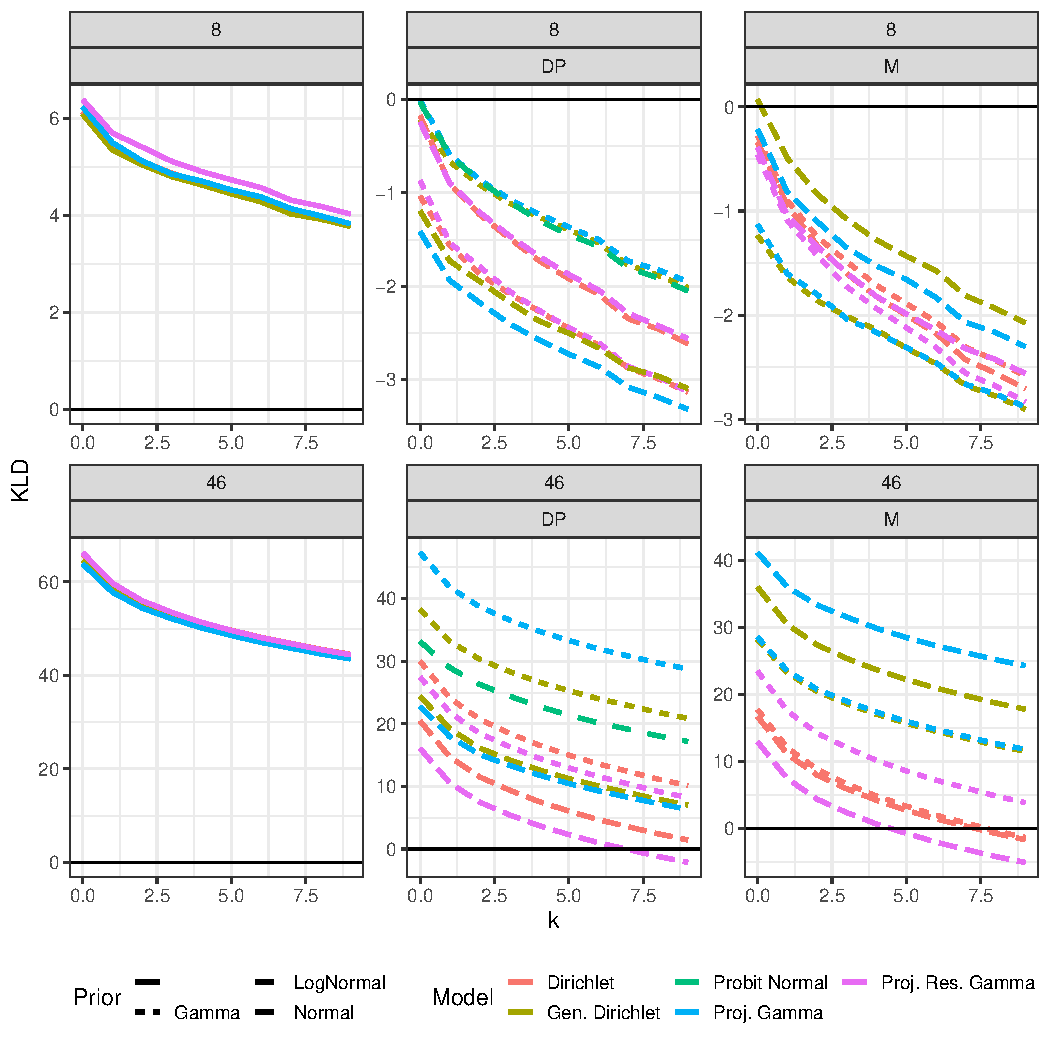
\includegraphics[width = 5in]{./images/kl_divergence_curves}
  \caption{KL Divergence Curves calculated through the KNN-KL Metric, evaluated between the empirical
  dataset and posterior predictive datasets of various models.  The top row corresponds to the
  8-dimensional data, while the bottom row the 46.  The left column corresponds to the vanilla models
  with no mixture method; the middle column a Dirichlet process prior, and the right column a finite
  mixture model.}
\end{figure}

Interpreting the KL divergence curves in Figure~\ref{fig:knnkl}, KL divergence at its core is a
  log-ratio of densities.  We would prefer, all else being equal, a KL divergence near 0.
  Interpreting this particular divergence metric, a KL divergence less than 0 means on average,
  that the $k$th closest sample from the posterior predictive dataset is closer to the observation
  than the $k$th closest sample from the empirical dataset.  There is a logged ratio of sample sizes
  to account for differences in cardinality between the empirical dataset and posterior predictive.

From this, we would interpret the \emph{best} model as that model which remains closest to the
  horizontal line at $0$.  For the 8-dimension model, this means the generalized Dirichlet and
  projected Gamma models, the unrestricted Gamma based models, seem to perform the best.   This is
  in stark contrast to our inference from the earlier posterior predictive loss and energy score
  criterions, which sharply favored the restricted Gamma models.  However, as dimensionality
  increases, we see that the restricted Gamma models again become favored, indicating that the
  greater flexibility of the unrestricted Gamma models becomes burdensome to fit in a
  high-dimensional case.



% EOF
